\documentclass[a4paper,oneside,11pt]{book}
%----------------------------------------------------------------------------------------
%	WELCOME!
%   It is probably worth having a read through this file to set up the broad parameters.
%----------------------------------------------------------------------------------------

%----------------------------------------------------------------------------------------
%	COVER PAGE
%   The cover page is laid out in title/title.tex. You can choose a colour
%   or black and white logo
%----------------------------------------------------------------------------------------

%----------------------------------------------------------------------------------------
%	THESIS INFORMATION
%   Put title, author name, degree, type of work, school, department in here
%   It will be used for the title page and for the embedded PDF information
%----------------------------------------------------------------------------------------

\newcommand{\thesistitle}{Internship Technical Report} % Your thesis title, this is used in the title and abstract
\newcommand{\degree}{Computer Science} % Your degree name, this is used in the title page and abstract
\newcommand{\typeofthesis}{Master in Integrated Computer Science} % dissertation, Final Year Project, report, etc.
\newcommand{\authorname}{Efeosa Eguavoen} % Your name, this is used in the title page and PDF stuff
%% Comment out the next line if you do not want your ID to appear
\newcommand{\supervisor}{Supervisor: Tim Fernando}
\newcommand{\school}{\href{http://www.scss.tcd.ie}{School of Computer Science and Statistics}} % Your school's name and URL, this is used in the title page


\AtBeginDocument{
  \hypersetup{pdfauthor=\authorname} % Set the PDF's author to your name
  \hypersetup{pdftitle=\thesistitle} % Set the PDF's title to your title
  \hypersetup{pdfsubject=\degree} % Set the PDF's keywords to your keywords
}

%% Language and font encodings
\usepackage[T1]{fontenc} 
\usepackage[utf8]{inputenc}
\usepackage[english]{babel}

%% Bibliographical stuff
\usepackage[round,sort,comma,numbers]{natbib}

%% Document size
% include showframe as an option if you want to see the boxes
\usepackage[a4paper,top=2cm,bottom=2cm,left=2cm,right=2cm,headheight=12pt]{geometry}

%% Useful packages
\usepackage{amsmath}
\usepackage[autostyle=true]{csquotes} % Required to generate language-dependent quotes in the bibliography
\usepackage[pdftex]{graphicx}
\usepackage[colorlinks=true, allcolors=black]{hyperref}
\usepackage{caption} % if no caption, no colon
\usepackage[parfill]{parskip}    % Begin paragraphs with an empty line rather than an indent
\usepackage{setspace} % to permit one-and-a-half or double spacing
\usepackage{enumerate} % fancy enumerations like (i) (ii) or (a) (b) and suchlike
\usepackage{booktabs} % To thicken table lines
\usepackage{fancyhdr}

\pagestyle{plain} % Embrace simplicity!

\renewcommand{\theequation}{\arabic{equation}} %% use continuous equation numbers

%% Format Chapter headings appropriately
\usepackage{titlesec}
\titleformat{\chapter}
{\normalfont\huge\bfseries}{\thechapter}{1cm}{} 

\titleformat*{\subsection}{\normalsize\bfseries}
\titleformat{\subsubsection}{}{\thesubsubsection}{1em}{\itshape\bfseries}

\title{\thesistitle}
\author{\authorname}

\frontmatter
\begin{document}
\begin{titlepage}

\center % Center everything on the page

%% All the text parameters should be taken from the start of the main.tex file.
%% You should only alter stuff here if you want to change the layout

%----------------------------------------------------------------------------------------
%	LOGO SECTION
%----------------------------------------------------------------------------------------
%% Choose one of the following -- a colour or black-and-white logo


\includegraphics{title/black.jpeg}\\[1cm] 
%\includegraphics[width=12cm]{title/black-stacked-trinity.jpg}\\[1cm] 

\Large \school\\[1.5cm] % Minor heading such as course title
\ifdefined\department
\large \department\\[1.5cm] % Minor heading such as course title
\fi

%----------------------------------------------------------------------------------------
%	TITLE SECTION
%----------------------------------------------------------------------------------------
\makeatletter
{ \huge \bfseries \thesistitle}\\[1.5cm] % Title of your document


%----------------------------------------------------------------------------------------
%	AUTHOR SECTION
%----------------------------------------------------------------------------------------

\authorname\\ % Your name
\typeofthesis\\
\thesistitle\\
\supervisor\\[2cm]

%----------------------------------------------------------------------------------------
%	DATE SECTION
%----------------------------------------------------------------------------------------

{\large \today}\\[2cm] % Date, change the \today to a set date if you want to be precise


%----------------------------------------------------------------------------------------
%	TYPE OF THESIS SECTION
%----------------------------------------------------------------------------------------
School of Computer Science and Statistics \\
O'Reilly Institute, Trinity College, Dublin 2, Ireland

\vfill % Fill the rest of the page with whitespace

\end{titlepage}
\pagenumbering{roman}
\section*{\Huge{Declaration}}
\vspace{1cm}
I hereby declare that this report is entirely my own work and that it has not been submitted as an exercise for a degree at this or any other university.

\vspace{1cm}
I have read and I understand the plagiarism provisions in the General Regulations of the University Calendar for the current year, found at \url{http://www.tcd.ie/calendar}.
\vspace{1cm}

I have also completed the Online Tutorial on avoiding plagiarism `Ready Steady Write', located at
\url{http://tcd-ie.libguides.com/plagiarism/ready-steady-write}.
\vspace{3cm}

Signed:~\rule{5cm}{0.3pt}\hfill Date:~\rule{5cm}{0.3pt}

\newpage

\onehalfspacing\raggedright %\raggedright turns of justification and hypenation

\tableofcontents
\newpage
%\setlength{\parindent}{0.5cm}
\doublespacing

\mainmatter
\chapter{Goals}

\section{Technological Goals}
\subsubsection*{Goal: Learn 1 new technology in asynchronous programming and successfully implement it in a task.}
\textbf{Goal Achievement: }  In terms of the accomplishment of this goal,  I feel I completed it and might have even somewhat overachieved.  I built a consumer that uses the Kafka asynchronous programming technology and also used HubSpot's in house queueing system TQ2 in a subsequent task to bring it to completion.\\
\textbf{Goal Evaluation: } This goal was somewhat difficult to accomplish as using Kafka isn't something that is necessary in every task.  To drive this goal to completion,  I specifically asked my team lead if I could work on a task that would allow me to gain some exposure to async technologies.  One of the initial problems was how complicated Kafka was as a system and how in-depth the documentation was.  I experienced some paralysis with getting started initially as there was so much to consider and I was over-thinking the task at hand.  To overcome this,  I sought some guidance from other members of my team that had previously worked on Kafka and asked them for some guidance in how to start.  This enabled me to be able to get a better idea of what the task I was doing actually was and how to use Kafka to accomplish the task. \\  
\textbf{Success Factors:}  The biggest thing that helped me to get this goal to completion was the help of my team mates. By making it clear with my team lead that I had an interest in async technology and wanted to work with it,  my team lead actively assigned me tasks that allowed me to learn more about it.  Using my team mates expertise and experience as a resource helped me drive this goal to completion as they gave me the blueprint to using Kafka and what pitfalls to watch out for which made the process much smoother. \\
\textbf{Goal Re-evaluation:} If I could change this goal,  I would've tried to get more exposure to TQ2,  which was the in house software used.  I used it only a few times during my time at Hubspot but I feel like I didn't get as deep an understanding into how it works like I did for Kafka. 


\subsubsection*{Goal 2: Develop my coding style to be compatible with the world of work to reduce time how long my pull requests are in review by understanding the coding practices at Hubspot}
\textbf{Goal Achievement: } In terms of accomplishment,  I don't feel I accomplished this goal to the fullest extent but I definitely made a lot of progress on this goal.  I learnt how to write clean,  maintainable code and about how to write code with others in mind. \\
\textbf{Goal Difficulty Evaluation:}  Overall,  I think this goal might have been slightly difficult as changing your coding style drastically, quickly is rather difficult and takes a long time to do than I had at the internship.  One of the biggest barriers to achievement in this goal was I had to rethink about how I write code and instead use patterns and such that were widely used as the code would need to be maintained by someone else who I may never meet months down the line,  so the code would need to be able to explain itself.  To solve this,  I actively took notes on my pull requests to see what I was getting pulled up on multiple times and made the active choice to prevent that when I was completing tasks.  By the end of my intership,  I realised the average time a task spent in pr had reduced by roughly 25\% and the comments in relation to coding style were much less frequent.  Whilst I couldn't incorporate everything into my coding style,  I could see I made serious progress and achieved my goal overall.\\
\textbf{Success Factors:} The biggest driver of success for me was the comments on my pull requests and reading 'Clean Code' by Robert Cecil. Using the core concepts in the book gave me the foundation to build off as well as alerting me to some of the mistakes I had been making up to this point.  The pull-request comments acted as a sort of positive reinforcement to give me a gentle remind me about certain things I had been slacking on. \\
\textbf{Goal Re-evaluation:} One thing I would change here is I would expand this out to testing also.  I learnt a lot about testing while at HubSpot but I feel I didn't learn as much about how to write good tests and such as much as I would've liked and this was sort of my weak point. 


\section{Soft Skill Goals}
\subsubsection*{Goal 1 : Be able to receive feedback and also give back constructive feedback in order to increase my growth as an engineer by giving me instruction in areas I may be lagging behind, whilst being able to give my team lead direction in how best I learn}
\textbf{Goal Achievement: } I think I achieved this goal completely.  By the end of my internship,  I had created a positive feedback loop between myself and my team lead and other members on my team,  thus creating an space that was open and judgement free that enabled us all to grow as engineers. \\
\textbf{Goal Difficulty Evaluation:} I think this goal was absolutely necessary and even perpetuated into my other goals as being able to give and receive feedback is important as an engineer in terms of growth as you need to be able to change your style and learn new things constantly due to the nature of the industry.  The goal wasn't difficult to achieve as at HubSpot there's a culture of growth and positivity around giving each other feedback and especially on my team as my team lead felt responsible for the growth of each member of the team, making it easier for me to achieve this goal.  One challenge I faced was accepting that the comments on pull-requests aren't there to attack your ability to code but are instead there to help you to write better code.  By being able to receive this type of feedback better and re-orientating how I thought about it,  it enabled me to realise faults in my own work and work on fixing them.  In terms of giving feedback,  I had weekly personal meetings with my team lead to discuss things in general.  In these meetings I focused on discussing how I work as a person and how my team lead can work alongside this to give me feedback and help me grow.  These meetings accelerated the achievement of this goal as I could continually practice giving good feedback as I could continually tune what I should say as I could see weekly what was and wasn't working.  \\  
\textbf{Success Factors:} The biggest drivers for success on this task were the weekly meetings with my team lead.  Having this pre-allocated time every week to give each other feedback made it that bit easier to discuss things as I knew that this space was made specifically to talk which created a mental break for myself \\
\textbf{Goal Re-evaluation:} If I could go back and change anything about this goal,  I would expand it so that I could also be able to give feedback on other engineers pr's as I felt this was something I didn't do enough and could improve on.  This would also have the added side-effect of being able to learn from the senior engineers in terms of how they write code,  which I could incorporate into my own style. 


\subsubsection*{Goal 2: Increase my networking skills by having at least 10 1:1’s with people on and outside my team to widen my network and learn more about other peoples progression in Hubspot}
\textbf{Goal Achievement: } I overachieved in terms of this goal.  I managed to meet over 15 people in the time I was there and grew my Linkedin connections by over 50 which I felt made this goal an overwhelming success.  \\
\textbf{Goal Difficulty Evaluation:} I felt like this was an easier goal to accomplish in relation to my other goals as setting up meetings with people at HubSpot wasn't difficult as there was already numerous things in place at HubSpot for meeting new people and as an intern,  the intern team did coffee meets with interns based on different teams around the world.  I didn't have  any obstacles in achieving this goal.  \\  
\textbf{Success Factors:} The coffee chats with the other interns were important in driving this goal to fruition as the platform to meet new people and such was already in place,  I just had to use it. \\
\textbf{Goal Re-evaluation:} If I could make an improvement on this goal if I could go into the past,  I would ask to talk with people that maybe aren't in the engineering teams so I could get a better idea of HubSpot as a company overall. 

\section{Major Takeaways}
From setting goals to achieve during my internship,  they helped me to guide my focus and also encourage new behaviours.  By actively trying to change how I code,  I found myself thinking more about how other people would perceive my code and what pitfalls they would point out.  Goal setting also helped me manage my tasks and prioritize them in-terms of what would drive my goals forward and what would take away from them.  I also found a sort of motivation from setting goals as I had something bigger I was working towards and felt a sense of pride when I took major steps towards fulfilling these goals.
\chapter{Weekly Reports}
\section{Week 9}
This week, I re-orientated back to working on the Kafka Consumer. I had shifted focus from it for a few weeks as my team was focused on leaving Code Red which required us all to focus on doing the Hublet based work. As it had been a few weeks since I had last looked at the consumer, I spent some time re-familiarizing myself with it and figuring out what was the next step from where I had previously left it. \newline This week I had a meeting with my team lead to discuss the crit-sit that had occurred. I got some reassurance from my team lead not to take it personally or whatever and to just focus on continue working to my capacity as these things tend to happen. 

\subsection{Reflection}
On reflection, I should have not left the kafka consumer so suddenly and written myself some notes on how to get started back on it when I returned to work on it as I spent a few days just re-reading my own code that could have been spent instead making some more progress on the consumer. Also, I realised how important it is to have a good team lead on your team that can provide you with reassurance and such when things don't go according to plan and can help you get back into the swing of things.
\section{Week 10}
The major task this week was to split up the task of making the whole consumer into smaller, actionable parts. After coming up with a plan of all the parts that needed to be done, I started on adding the filtering logic to the consumer to check what sort of message is being sent for processing. This wasn't too difficult and was completed and sent to pr by the end of the week. \newline This week I had a 1-1 meeting with an intern on the security team in the states. It was interesting getting to see what other sort of projects interns get to work on at HubSpot and also advanced my goal of meeting new people and expanding my network.

\subsection{Reflection}
In hindsight, splitting up the tasks for the kafka consumer definitely helped me to speed up the process of getting it done as I had more focus on what I was doing each week and helped me to narrow in on what was important and not to get caught up trying to get it all to work all in one go. 
\section{Week 12}
This week, the primary focus was to create the function that would create the request body that would then be placed as part of the request to be sent to one of the endpoints. For this, I used a builder pattern as other classes have similar methods so I reused some of the code in those classes and just tweaked it for use here. Testing this change wasn't particularly difficult as it was just a matter of doing a series of asserts on the different fields in the class. \newline This week, a new intern joined the team. I was instructed to kind of show him the different products our team is responsible for and what our team mission is.

\subsection{Reflection}
The new intern joining my team really gave me some perspective on how far I had come from when I started at HubSpot. A lot of the things that I had struggled with initially like getting to grips with the different tools and the code base I no longer had issues with but could even show another person tips and tricks I had learnt from using them. This really helped me to put my growth into perspective. 
\section{Week 13}
This week the major thing I worked on was writing the endpoints that the kafka consumer would hit to send data to the database. There were some examples of endpoints in the database already so I could use those as a sort of framework for the 2 new endpoints I was introducing. I initially had some issues with verification but I switched the endpoints to become internal and that solved a lot of the issues. \newline This week there was a talk from the CTO of HubSpot, Dharmesh Shah. All the interns were invited to hear him speak and it was really interesting hearing about how HubSpot came about as he was one of the co-founders of the company. 

\subsection{Reflection}
I think the way I wrote the endpoints could have been more robust. While it's secure and will work, I thought the code was slightly messy as I rushed through it slightly as I wanted to move on to something else. The testing for this also wasn't as thorough as I'd have liked, I only wrote a series of unit tests and didn't perform an integration test with the other components. 

\section{Week 14}
The final part of the consumer I wrote this week, the wrappers for the endpoints. The wrappers were there for re-usability so other classes could reuse the endpoints as necessary. The testing for these wrappers was kept minimal as they were just code covering the endpoints that were previously tested. 

\subsection{Reflection}
This week I learnt about why having wrappers and such is so important. Having proprietary methods to access frequently used endpoints and such can really cut down on code duplication and also it makes it a lot easier to integrate into other projects as you can just use a builder pattern to create your request. 

\section{Week 15}
The main focus of this week was to do some thorough testing of the consumer from end to end. While each of the individual parts were working as intended, a full end to end test was necessary to make sure it worked as intended for users. Some bugs were encountered while writing the consumer which took a while to fix. \newline This week our team also rebranded from Flagship Integrations to ERP-Strategic Integrations as the focus of our team and our vision was shifting to be more of a toolbox for having the core processes needed to keep companies running. 

\subsection{Reflection}
This week, I learnt about how important the different types of testing are. If I hadn't done the end to end testing, I wouldn't have found some of the bugs in the code that I had encountered. Unit testing is fine when you're only working on smaller changes and not on larger systems, but using a mixture of unit testing, integration testing and end to end testing is the best way to make sure a system is tested exhaustively. 

\section{Week 16}
For my final week, I spent the majority of it doing clean up on the consumer and handing off my remaining tasks to my team mates. Whilst I had completed the consumer, there was still some other work remaining for making line items editable I couldn't get to so I transferred this on to the team to see it to completion. 

\section{Final Reflective Diary}
From working at HubSpot, I've learnt a lot about what it's like to work and be part of a team. Some of the major takeaways from the internship are as follows: 

\subsection{Ask Questions}
One of the most important things I've learnt over the course of the internship is how important it is to ask questions. When you start working at a new company with a new set of tools, a whole new code base it can be quite overwhelming. My first instinct was  to try tough it out but this was a mistake, I should have asked for help sooner which would have helped me on ramp sooner. I learnt that taking a small amount of time like 30 minutes or so to attempt things myself and then asking for help is the best way to get things done and moving as I would know enough to be know what questions to ask that would unblock me.

\subsection{Get Familiar With The Tools}
This was something I found incredibly useful and helped me to increase my productivity. Being comfortable with my development tools and learning the different IDE shortcuts saved me a few minutes constantly which added up over the course of the internship.

\subsection{Taking Responsibility For Your Work}
A major thing I found to be important was taking ownership of your work and being the one responsible for it. Being an intern it's easy to fall into the misconception that what you do doesn't really matter and you can make mistakes and nothing will happen, but this is a big misconception. I found that from breaking things that the work I do does have a real impact on our customers and that it goes beyond me with whatever I do. It's important to own up when you make mistakes and participate in conversations at work as you're part of the team and aren't treated differently just because you're an intern. Taking pride in your work and executing to the full extent of your ability is a good way to show ownership.

\subsection{Ask For Feedback}
At HubSpot, I had weekly meetings to give and receive feedback from my manager that was invaluable to my growth over my time there. Feedback is imperative to your growth as you often don't know in what sectors you may be lacking and in what sectors you may be strong in. Feedback is a great way to figure this out. While not all feedback is positive, not taking it personally and understanding you're being told this as your manager wants you to grow and be the best engineer you can be is important.

\subsection{Setting Goals}
The course of an internship is over quite a long time so it can be quite difficult to stay on track and you can drift somewhat and stagnate. Having goals and things you're working towards can keep you on track and keep you focused. Taking active steps towards your goals can help you grow faster and will keep you motivated as you work.
\chapter{Executive Summary}

\section{Executive Summary}

During my time at HubSpot I was assigned 2 major tasks that I worked on over the course of the few months of my placement. To get me started and introduced to the tech stack at HubSpot, I first started with an onboarding project that enabled me to become somewhat familiar with the stack by using many of the major tools and languages that are commonly used in HubSpot. This introductory project introduced us to the major programming languages in HubSpot, some of the predominant patterns used at HubSpot such as the Builder pattern and how to use things like annotations and dependency injection. There was also an aspect of the onboarding that required us to build a react app and create a front end that plugged into a simple backend we had created also. This wasn't a part I spent too much on as I was on a predominantly back-end team.\newline \\ Once I had completed this, I was introduced to my first major task, building a multicurrency consumer to make currency fields editable in the UI. This was part of a wider set of changes to multiple repositories my team owned to standardise fields so we could make the prices of items and such editable in the UI, which was a major pain point for our customers. This change was quite large in size and required multiple pull requests and a lot of code to be written to get it going. For this change to be made, some endpoints had to be written alongside a brand new kafka consumer. This task was what I spent the majority of my time at the internship working on. \newline \\The other task I worked on during my time at HubSpot was a change to users using Shopify as part of a company wide initiative to make us GDPR compliant. In order to do this, a new EU Hublet was made as previously all data was routed to the US and handled there but under GDPR, users have to be allowed to both chose where their data is sent and where it's stored. To make us GDPR compliant, I had to change the webhooks for all users using Shopify to point to a load balancer that would then determine where the data should be routed. To do this I had to write a backfill job that performed some major operations on the database and changed the data in there. This change was fairly straight forward but there was a bug that made it to production that caused all users webhooks to be broken. This bug was fixed and the task was re-run but there was a period of down time that took a period of remidiation to fix and retrieve all missed data that couldn't be synced while the webhooks weren't active.
\chapter{Project 1: Multi-Currency Consumer}

\section{Introduction}
During my time at HubSpot I was assigned 2 major tasks that I worked on over the course of the few months of my placement. To get me started and introduced to the tech stack at HubSpot, I first started with an onboarding project that enabled me to become somewhat familiar with the stack by using many of the major tools and languages that are commonly used in HubSpot. \\ Once I had completed this, I was introduced to my first major task, building a multicurrency consumer to make currency fields editable in the UI. This was part of a wider set of changes to multiple repositories my team owned to standardise fields so we could make the prices of items and such editable in the UI, which was a major pain point for our customers.\newline \\ When I was first presented with this task, I thought it would be fairly simple as on the surface, it seemed like simply getting what type of multicurrency change is being made and then just adding the field to the database. Once I had gotten started, it became much more complex and required multiple steps and code refactors whilst the project was being built. \\ For example, when a user makes a change to a multicurrency to their HubSpot portal, the consumer would then process what type of change was made (addition/deletion being the only two the conusmer was concerned with) and from there, the consume would create a a HubSpot standardized field and place it into the database for the user alongside other fields such as the label to be displayed in the UI in the case of an addition and in the case of a deletion, the consumer would remove the corresponding fields from the database. \newline \\ This change seemed pretty simple but there's multiple hidden requirements that aren't immediately obvious. For instance, what should be done for all the multicurrencies that are already in a user's portal? What should be in the case where a user doesn't yet have any multicurrencies in their portal and decides to add one? How are calls to/from the database to be handled? Questions like these and many others needed to be answered and dealt with before and during the coding process. \\ Luckily for me, my team had started some of the necessary work making it easier for me to get to coding. For instance, my team already had created the Kafka producer and set up much of the infrastructure so I just had to work with it to do complete this task.

\section{Design Approach and Architecture}
To complete this task, I split the overall task into multiple subtasks to be completed:
\begin{itemize}
\item Standardized Multicurrency labels and fields Generator
\item Build Kafka Consumer
\begin{itemize}
\item Filter Kafka message into Add/Delete
\item Pre-build request body for processed message
\item Send request
\end{itemize}
\item Create Internal Endpoints for adding/deleting multicurrencies
\item Build Wrappers for hitting endpoints to be used by Kafka Consumer
\end{itemize}

I went with a top down approach initially when defining each of the individual components and fleshing out components as I went along. I decided to use this as I was sure there may be some hidden requirements that may arise during the coding process. Also, the top down approach to software engineering is much more requirements driven and was more in-line with clean code practices as I could avoid writing code I may not need. For some of the individual components, I did go with more of a bottom up approach like the kafka consumer, as this consumer could be reused for something elsewhere with some changes to the functionality. \newline \\ For the overall architecture, I went with one of the more common design patterns, the \textbf{Model-View-Controller (MVC)} system. I went with MVC due to the scalability it provides alongside the support for asynchronous techniques like Apache Kafka which is a major framework in use at HubSpot.

\begin{figure}[ht]
  \centering
  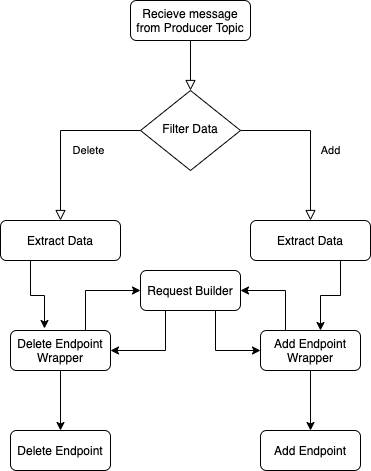
\includegraphics[scale=0.7]{multicurrency/multi.png}
  \caption{Flow Diagram of Architecture}
\end{figure}

\subsection{Model-View-Controller (MVC)}
MVC is a common architecture pattern used in web based applications. MVC separates out the layers of business logic and data interactions(model) from the presentation(view) and intermediary between the two layers(controller). This pattern is so popular as it decouples each of the major aspects of the design from each other and is also highly scalable due to how modular the design is.


\subsubsection{Model}
The data and business logic of the application are wrapped in the model layer.
It's frequently made up of a number of interconnected domain objects.
The models represent the nouns or entities in the system, such as user or order, and interact with any of the other layers of the system.  
\newline The model layer, on the other hand, includes not just models but also validators, methodologies, and any other element that directly affects or distorts the underlying data of the application. \newline \\ 
Each model has a user interface that reflects the logical functions that can be performed on the data it represents.
An illustration of the capabilities contained in an application's model layer: A \textit{FullName} method on a User class returns a merger of the first and last names associated with the user it depicts. The same object also has an \textit{UpdateName} function that updates the corresponding name in the database. The same object could then use a Validator instance to make sure none of the fields are empty before being placed into the database.  \newline \\
The model Layer often utilises some form of \textbf{Object Relational Mapping},  which is a layer of abstraction which is designed to transfer data from the the scalar values used in database storage to the objects used in object orientated programming languages and vice versa.  While a traditonal SQL database is used in many instances,  noSQL databases and/or web services that perform some sort of data persistence could be used as the database layer instead. 
\newline In many versions of the model class,  a set of static methods which utilise the ORM to search for and instantiate instances of the model.
\subsubsection{View}
The 'View' layer is responsible for the visual layer of the model.  This represents the graphical user interface a user may interact with. Views perform as the output of the system, whereby data from the model is represented.  In many MVC architectures,  the view is sensitive to changes in the data held in the model and hence self updates to reflect any new changes in the data.  The view itself does not transformations or alterations of the data itself,  it just acts as thin layer between the model and the controller.  Data from the user may be inputed in the view layer but is ultimately sent to the controller to be dealt with.
\subsubsection{Controller}
The controller layer is primarily responsible for processing user input.  A controller normally has a 1-to-1 relationship with a view or a 1-to-many relationship with a series of views.  When a user inputs data via an interface in the view layer,  this triggers an event to occur which is dealt with by the controller layer. The controller layer could for instance instruct the view layer to resize itself if a user resizes the size of the input window.  Another example is to update the data in the model and hence update the view layer if a user inputs new data into the view layer initially.  Controllers have permissions to frequently access the model layer and re-construct and transform the data in that layer.

\begin{figure}[ht]
  \centering
  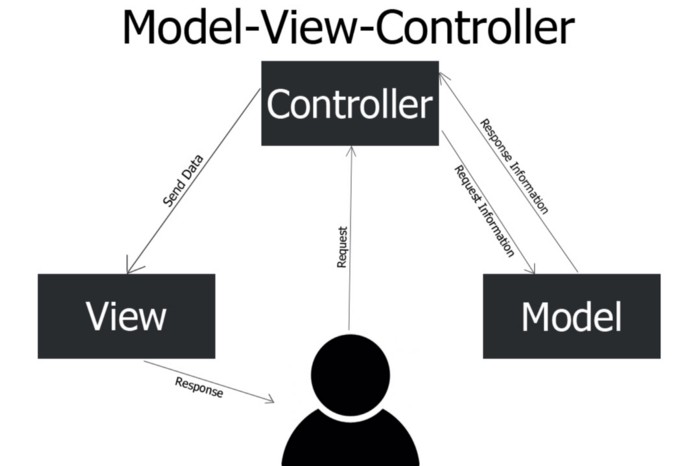
\includegraphics[scale=0.35]{multicurrency/mvc.jpg}
  \caption{Model-View-Controller overview}
\end{figure}

\section{Implementation}
For the implementation of this task, it was split into multiple sub-tasks with each part being tested individually before the next part was created.
\subsection{Standardized Labels and Fields Generator}

The first task I worked on was creating a function that would take in some multicurrency and then convert it to a HubSpot standardized field. \newline For example,  the function would take in a currency like \textit{USD} and then return it in the form \textit{hs\_external\_price\_USD}.  \newline Initially this change was simple to write as it required only the name of the currency that is being used to create the field according to the ISO 4217 standard.  \newline \\ As work progressed on this function,  it was refactored slightly and given some more utility to be able to generate more fields that had to do with multicurrencies.  A function to create the internal version of the fields was also created alongside the labels that would be displayed in the UI on the page in a users portal where multicurrencies would be managed.  \newline This task took some time to get to production as there was a number of comments on the pull requests that needed to be implemented as it was my first major pr.  This change showed me how to write code according to the level that's expected at HubSpot.

\subsubsection{Problems} 
The major problem that arose was that for some 3rd party developers didn't use the ISO 4217 standard for the currencies so matching them in the syncing engine wasn't possible.  \newline To get around this issue,  we first of all had to check if the inputted multicurrency was ISO 4217 compliant and then from there would generate the field.  Any input data that was not compliant would then return an error.

\subsubsection{Testing}
In terms of testing for this change,  I wrote a series of unit tests to test the different expected behaviours of this change.  The tests were written in advance of the code being written as at HubSpot test-driven development is a big thing and is greatly encouraged. 

\subsection{Kafka Consumer}
The next task I worked on was creating kafka consumer to consume messages from the kafka producer queue. This was a much larger task than the previous task so I split it up into smaller pieces to make the task more manageable. This aspect of the task would fall into the ''Controller'' layer of the MVC framework as all data operations are performed here before being sent to the database or 'Model'

\subsubsection{Building The Base Consumer}
The base kafka consumer was constructed from an interface for building kafka consumers that was already pre-created. The consumer was subscribed to a topic that was responsible to publish messages concerning multicurrency updates from a producer. When a message gets published to the queue, the kafka consumer would then grab the message from the queue and then process it accordingly. 

\subsubsection{Filtering Kafka Messages}
The next major part of the consumer I wrote was to grab the type of request in the message and from there, process the message accordingly. To process the message, I used a switch statement to filter the data based off the type in the message body. The currency being updated in question is then also extracted from the message body.

\subsection{Pre-building The Request Body}
Once the major aspects of the request has been collected from the message body, the request body is then created. The label's, standardized fields and such are all created here.

\subsubsection{Sending the Request}
Once all the previous steps have been completed, the request is then sent to the corresponding internal endpoint, using the previously built request body. 

\subsubsection{Problems}
One of the major problems in creating this consumer was figuring out how to prevent messages being processed twice. Luckily, kafka has numerous guarantees that ensure that each message is processed exactly once making this a none issue. Another issue was figuring out how to scale this to work on a large scale. To solve this issue, kafka enables multiple kafka workers to be subscribed to a topic so more workers can be spun up as necessary or killed as traffic changes. 

\subsubsection{Testing}
To test this change, a number of integration tests were written to make sure each of the core components interacted with each other as necessary. As each of the individual components do different things, unit testing the overall system wasn't possible. Each of the individual components were unit tested as necessary. One bug that was encountered in testing was getting the correct multicurrency field from the topic. To fix this issue, I had to re-parse the data given from the topic into ISO 4217 compliant fields.

\subsection{Endpoints}
The next major component that needed to be written was the internal endpoints that would hit the database and update the data in there. This would compromise part of the 'Model' aspect of the MVC framework as it's responsible for framework operations. The endpoints needed to be internal as we didn't want to expose them to external developers and also it allowed us to use the '@internal' annotation to allow it to be secure by using Oauth. \newline \\ To create the endpoints, a path was first defined for both the add and delete endpoints in seperate functions. From here, we could then hit the database directly using some ORM methods. This component didn't take much time to create as it was a relatively easy aspect to code as it was basically a partial implementation of a REST api. \newline \\ The endpoints that were created were  \begin{itemize}
\item An 'Add' endpoint to create a multicurrency field mapping in the database
\item A 'Delete' endpoint to remove multicurrency field mappings in the database
\end{itemize}

\subsubsection{Problems}
One issue that I faced writing this was dealing with verification as I had initially planned on creating an open endpoint and hitting it as necessary. But I kept getting errors due to verification due to the fact I was trying to hit internal database's via external calls. To solve this, I made the endpoints internal which enabled stopped these errors from appearing as Oauth was used for verification automatically so I didn't need to worry about security.

\subsubsection{Testing}
To test this change, I did some integration testing instead of End-to-End testing as external users wouldn't have access to this endpoint so all that mattered was that it performed according to the parameters we expected. I did some asserts on the expected response from the endpoints, and mocked out the calls to the database as this was beyond the scope of the test. 


\subsection{Wrappers for Endpoints}
The final part to complete this task was to write some wrappers around the endpoints defined above.  Whilst the endpoints could be accessed without wrappers,  to make the code cleaner,  more maintainable and also more reusable,  creating api wrappers was the best choice.  \newline
This code addition was also rather small,  all that was necessary was to create functions that would take in the request from the kafka consumer and then send them to endpoint where they'd be dealt with.  These functions acted as part of the 'Controller' aspect of the MVC architecture.  \newline \\ For testing and problems encountered, since this wasn't a huge change, no real problems were encountered whilst writing these wrappers. 

\section{Evaluation and Testing}
Once all the parts of the consumer had been created,  testing the entire flow of the system became top priority.  Whilst each of the individual parts were unit tested and integration tested,  an end-to-end test of the entire system could only be done when the entire thing was assembled.  \newline \\ To test the entire system,  using Orion,  a branch deploy was done of the code base including this consumer to the staging environment.  Next,  all active Kafka consumers subscribed to this topic in staging were temporarily paused to test this change to prevent a flood of errors being sent in case the change had some bugs.  Finally,  testing was done using a test portal. \newline To begin testing,  I started with testing adding new multicurrencies.  To evaluate if the change worked,  I searched the logs for https requests and checked if they were going to the correct services.  Finally,  I checked the database to see if the new fields were added to the test portal.

\subsection{Deployment}
\begin{figure}[ht]
  \centering
  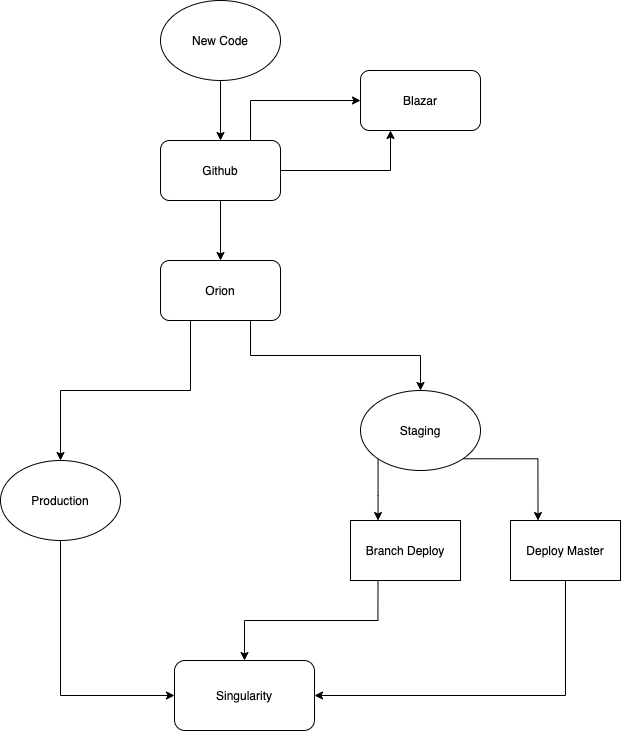
\includegraphics[scale=0.7]{multicurrency/deployment.png}
  \caption{Flow Diagram of Architecture}
\end{figure}
\subsection{Problems encountered}
One issue I found while testing was I saw requests were not going to the correct services but were ending up somewhere completely different.  I initally checked my code to debug it but I couldn't seem to figure out what was going wrong.  Next I ran the kafka worker locally to find out what was wrong as I could debug it step by step as new requests came in, but again I couldn't figure out what was wrong.  I finally asked my Team Lead for assistance,  it turned out that because I was testing in Staging,  the route requests take is slightly different as there are 2 streams in Production to deal with all the traffic while in Staging there's only 1 as it's just for testing.  I was expecting the route of traffic to match Production but it turned out the testing was working as intended,  my assumptions were just wrong. 

\section{Analysis and Possible Changes}
Using the MVC framework was very useful in structuring how the code should be written and how to create tasks and assigning their importance.  Using this framework also allowed for a high degree of scalability as each of the parts of the consumer work independently of each other which has the added benefit of easier maintenance as if any part breaks, there's no effect on the other parts of the code.  \newline In terms of changes I would make if I could go back now, I would restructure how I created the endpoints.  Whilst they worked as intended, the testing for them was somewhat fragile due to how I wrote the code for the endpoints.  Malformed inputs could cause some errors or if the fields haven't been properly verified before being inputted errors could occur.  While this isn't an issue at the present time as it's an internal API,  if it were to ever become open to 3rd parties,  it would need to be re-written to be more robust and do more error checking.

\end{document}